\documentclass[runningheads]{llncs}
\usepackage[UTF8,scheme=plain]{ctex}
\usepackage{amsmath,amssymb,booktabs,multirow,graphicx,xcolor,hyperref,array}
\usepackage{caption}
\usepackage{float}
\usepackage{tikz}
\usetikzlibrary{arrows.meta,positioning,fit,calc,backgrounds}
\usepackage{enumitem}
\setlist{nosep,leftmargin=2em}
% 将 Markdown 风格反引号转换为等宽文本，并保护文件名中的下划线。
\catcode`\`=\active
\def`#1`{\texttt{\detokenize{#1}}}
\graphicspath{{figures/}}
\hypersetup{colorlinks=true,linkcolor=blue,urlcolor=blue,citecolor=blue}
% 图注独立于正文排版，便于快速辨识编号与说明。
\renewcommand{\figurename}{Figure}
\captionsetup[figure]{font=small,labelfont=bf,labelsep=period,
  justification=raggedright,singlelinecheck=false,skip=6pt}
\captionsetup{hypcap=false}
% 放宽浮动体的排版边界，避免短图表被单独推到空白浮动页。
\renewcommand{\topfraction}{0.92}
\renewcommand{\bottomfraction}{0.88}
\renewcommand{\textfraction}{0.08}
\renewcommand{\floatpagefraction}{0.72}
\setlength{\textfloatsep}{12pt plus 3pt minus 3pt}
\setlength{\floatsep}{10pt plus 3pt minus 3pt}
\makeatletter
\setlength{\@fptop}{0pt}
\setlength{\@fpsep}{12pt}
\setlength{\@fpbot}{0pt plus 1fil}
\makeatother
\setlength{\emergencystretch}{2em}

\newcommand{\method}{M1}
\newcommand{\full}{FullSchema}
\newcommand{\schemarag}{SchemaRAG}

\title{Budget-Aware Dynamic Schema Adaptation for Efficient LLM-Based Information Extraction}
\titlerunning{Budget-Aware Dynamic Schema Adaptation}
\author{作者信息待补}
\authorrunning{作者信息待补}
\institute{Northwest University, Xi'an 710127, China}

\begin{document}
\maketitle

\begin{abstract}
异构文化遗产记录的信息密度和可抽取字段并不均匀，固定使用完整 Schema 会为低信息记录
引入无效字段负载。本文考察能否利用完整 Schema 抽取产生的模型辅助银标监督，在调用前按记录
选择字段，并将字段价值先验和估计字段成本纳入预算约束的动态 Schema 构造。我们以字段选择
完整性而非字段值事实正确性评价裁剪代价：在 500 条模型辅助评价参考记录的 476 条共享成功子集上，`budget-200`
覆盖 83.03\% 的参考非空字段，选择阶段缺失率为 16.97\%。以 100 条银标记录启动训练后，
在不与该评价集重叠的 2,000 条开发性能负载上，`budget-200` 在 Qwen3-8B-AWQ~\cite{yang2025qwen3} 服务和
单进程有界队列条件下，较完整 Schema 呈现更少的总 Token、更短的在线流水线时间和更高的
有效吞吐。补充诊断表明，Token 下降主要来自字段数缩减，现有加权排序未稳定优于等权、频率或
简单 Top-$k$。因此，本文的结论限于当前数据、模型服务和单进程配置下，预算约束可实现字段
负载控制及其可量化的完整性代价，不支持排序最优性、独立泛化或生产级扩展性结论。
\end{abstract}

\keywords{文化遗产抽取 \and 动态 Schema \and 大语言模型 \and 预算约束 \and 数据预处理 \and 在线吞吐}

\section{引言}

文化遗产数据库通常长期汇集自多个来源，记录在键名、描述长度、信息密度和可抽取字段上差异
显著。对每条记录发送完整 Schema 虽然简化了调用逻辑，却会使低信息记录携带大量无效字段定义，
增加输入 Token、输出 Token 和在线推理时间。在大规模预处理场景中，固定 Schema 负载可能成为
运行瓶颈；本文不对数十万条记录规模的端到端性能作实证推断。

已有结构化信息抽取和检索增强研究表明，大语言模型能够按照给定 Schema 输出字段值，并可依据
输入内容缩小候选 Schema。然而，选择过少可能遗漏长尾字段，选择过多又会重新引入 Schema 负载。
对于缺乏大规模人工字段标注的文化遗产记录，尚不清楚少量由完整 Schema 抽取生成的模型辅助银标
监督，能否为调用前的字段裁剪提供足够信号。本文因此考察两个问题：记录级字段选择能否在模型
辅助参考集上保持较高的字段覆盖，并在包含排队、请求、重试和结果写入的端到端流水线中降低运行
时间、提高有效吞吐？

为回答上述问题，本文将记录级字段选择建模为预算优化，利用稀疏文本特征预测字段存在性和输出
长度，再结合字段价值、估计成本与必选字段约束生成动态 Schema。实验以 FullSchema 作为既有抽取
行为参照，并与基于 embedding 的固定 Top-$k$ 字段检索进行比较。本文所称预算是字段组合阶段的
估计容量，而非最终 API Token 或货币成本上限；字段覆盖仅评价选择集合，不检验字段值的事实正确性。
本文不构建人工 Gold，结论也限于当前数据、模型服务、Prompt 和单进程流水线条件。

\section{相关工作}

LLM 结构化抽取工作如 ChatSchema~\cite{chatschema}、UIE~\cite{uie} 和
InstructUIE~\cite{instructuie} 通常假设目标 Schema 已确定并直接提供完整字段。SchemaRAG~\cite{schemarag}
依据记录与 Schema 元数据的语义相似度检索固定 Top-$k$ 字段；PARSE~\cite{parse} 和 Schema-adaptable
Knowledge Graph Construction~\cite{adakgc} 分别关注 JSON contract 与全局 Schema 演化。本文的适配点是
在候选字段相对稳定时做记录级调用前选择，新增组合则是将银标行为预测、字段价值和估计成本接入预算选择器。

预算感知抽取、路由和 Prompt 压缩工作（Doctopus~\cite{doctopus}、FrugalGPT~\cite{frugalgpt}、
LLMLingua~\cite{llmlingua}）从方案、模型或文本 Token 层面控制开销；本文不改变模型或连续文本，
只在同一服务前选择字段。文中的 SchemaRAG 是依据公开描述实现的固定 Top-$k$ 外部适配，不代表
官方实现或完整系统的性能上限。LLM serving 优化如 PagedAttention~\cite{pagedattention} 作用于 KV-cache；
本文的单进程 Producer--Consumer Runner 不改动服务引擎，仅测量字段裁剪对请求负载、完成时间、
吞吐和尾延迟的影响。Huang 等~\cite{huang2023} 提供数字文化遗产结构化管理背景，本文不据此推导
跨数据集或生产规模结论。

\section{问题定义与总体流程}

设原始记录为 $r$，候选字段集合为 $F$，字段选择结果为 $S_r\subseteq F$。对字段
$f$，选择器预测其存在性分数 $p(r,f)$ 和输出 Token 数 $\hat{o}(r,f)$。字段价值
权重 $w_f$ 是可审计但未由当前数据学习为最优解的任务启发式先验，字段定义成本为 $d_f$。
动态选择写为：
\begin{equation}
 u(r,f)=p(r,f)w_f,
 \qquad c(r,f)=d_f+\hat{o}(r,f),
 \label{eq:utility-cost}
\end{equation}
\begin{equation}
 \max_{S_r}\sum_{f\in S_r}u(r,f),
 \quad \text{s.t.}\quad \sum_{f\in S_r}c(r,f)\leq B.
\end{equation}

其中 $B$ 是字段选择阶段的估计字段成本容量，不是 LLM 调用的端到端 Token 上限或货币
成本上限。最终 Token 还包括原文、固定 Prompt、实际输出和重试消耗。

如图~\ref{fig:overall-framework}，离线阶段由 FullSchema 银标训练 M1；在线阶段依次完成记录序列化、
字段预测与预算选择、动态 Schema 构造、并发 LLM 调用和结果写入。

\begin{figure}[!ht]
\centering
\resizebox{\linewidth}{!}{%
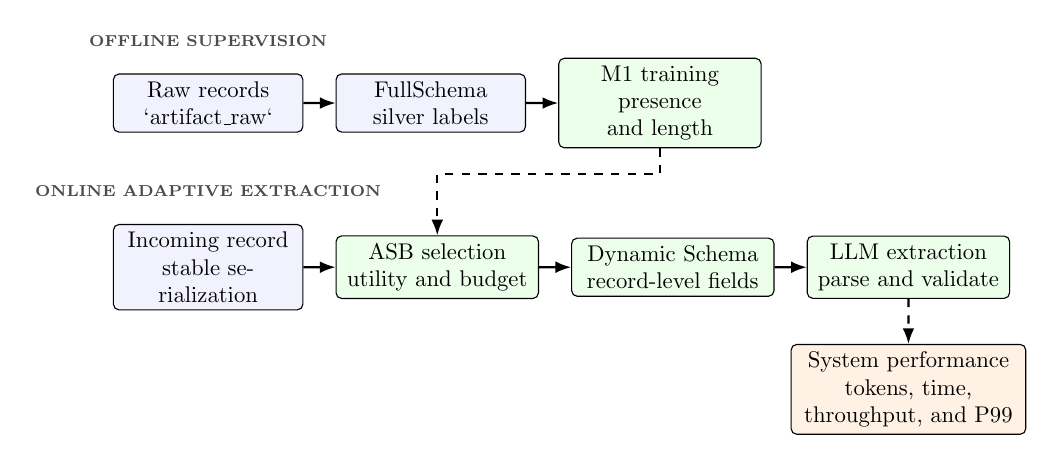
\begin{tikzpicture}[scale=0.82,transform shape,
  node distance=5mm and 5mm,
  data/.style={draw, rounded corners=2pt, align=center, minimum height=9mm,
    text width=27mm, fill=blue!5},
  process/.style={draw, rounded corners=2pt, align=center, minimum height=9mm,
    text width=29mm, fill=green!8},
  eval/.style={draw, rounded corners=2pt, align=center, minimum height=9mm,
    text width=34mm, fill=orange!10},
  stage/.style={font=\bfseries\scriptsize, text=black!70},
  arrow/.style={-{Latex[length=2mm]}, thick},
  dependency/.style={-{Latex[length=2mm]}, thick, dashed},
  evalarrow/.style={-{Latex[length=2mm]}, thick, dashed}
]
\node[stage] (offline-title) {OFFLINE SUPERVISION};
\node[data, below=3mm of offline-title] (raw) {Raw records\\`artifact\_raw`};
\node[data, right=of raw] (silver) {FullSchema\\silver labels};
\node[process, right=of silver] (train) {M1 training\\presence and length};
\draw[arrow] (raw) -- (silver);
\draw[arrow] (silver) -- (train);

\node[stage, below=7mm of raw] (online-title) {ONLINE ADAPTIVE EXTRACTION};
\node[data, below=3mm of online-title] (record) {Incoming record\\stable serialization};
\node[process, right=of record] (select) {ASB selection\\utility and budget};
\node[process, right=of select] (schema) {Dynamic Schema\\record-level fields};
\node[process, right=of schema] (llm) {LLM extraction\\parse and validate};
\draw[dependency] (train.south) -- ++(0,-4mm) -| (select.north);
\draw[arrow] (record) -- (select);
\draw[arrow] (select) -- (schema);
\draw[arrow] (schema) -- (llm);

\node[eval, below=7mm of llm] (performance) {System performance\\tokens, time, throughput, and P99};
\draw[evalarrow] (llm.south) -- (performance.north);
\end{tikzpicture}%
}
\caption{Overall study design. Raw records construct FullSchema silver-label supervision for M1
training. The online path applies ASB selection before dynamic-Schema extraction. Evaluation reports
model-assisted reference-field coverage and system performance; the reference is not independent
human factual Gold.}
\label{fig:overall-framework}
\end{figure}

\section{数据与监督信号}

项目数据库中的原始记录表 \texttt{artifact\allowbreak\_raw} 与完整抽取结果表
\texttt{artifact\allowbreak\_extract} 通过唯一标识 `artifact_id` 对齐，内连接得到 6,763 条记录，
并划分为训练集 5,410 条、验证集 677 条和测试集 676 条。本文仅考虑 18 个预定义目标抽取字段，
而非原始 JSON 中任意可见的键；`artifact_id` 仅用于连接、划分和结果配对，不作为模型输入。性能负载
中的记录类型比例与源库的最大偏差约为 1.4 个百分点，但原始记录通常仅含 5 个非空字段，因此结果
不主张覆盖所有来源分布。

为检查模板级重复，采用字符 3-gram Jaccard 相似度阈值 0.6 扫描性能负载，发现 1,101 对近重复记录
和 111 个近重复簇，最大簇包含 50 条记录，并构造 132 个类型--年代代理分组。这些结构被保留，以
反映目标数据分布；结果不解释为跨模板或跨来源的独立泛化证据。

候选 Schema 含 18 个目标字段，其中 `name` 与 `category` 为必选字段，`desc` 采用常量存在性预测，
其余字段由选择器按记录决定；多个长尾字段的银标非空率低于 2\%。字段权重是可审计的任务配置，而非
学习得到的最优权重，完整定义见随稿材料。FullSchema 使用全部字段，动态 Schema 选择子集
$S_r\subseteq F$。`artifact_extract` 是 FullSchema 产生的 model-assisted silver reference，而非
人工真值：字段非空性构成 `present` 标签，非空值经 OpenAI 的 `cl100k_base` tokenizer 计数后构成
长度标签。因此，M1 学习的是 FullSchema 输出行为，而非经独立人工确认的事实真实性。


\section{方法实现}

\subsection{基于稀疏文本特征的字段预测器}

原始 JSON 键值和描述文本稳定序列化为 `record_text`。字段 $f$ 的标签
$y_f(r)$ 取其 FullSchema 银标是否非空；非空值经 `cl100k_base` 编码后的长度作为输出长度监督。
训练、验证和测试按 `artifact_id` 隔离，验证集仅校准阈值。各字段使用独立的平衡逻辑回归分类器；
长度分支拟合 $\log(1+o_f(r))$，正例不足时回退至中位数。

M1 拼接字符级和词级 TF--IDF，输出 $p(r,f)$ 与 $\hat{o}(r,f)$；字符模型仅作基线。M2 分别训练
两类特征并线性融合概率，只作离线消融。词表仅在训练子集拟合；训练规模
$n\in\{50,100,250,500,1000,2500,5410\}$，采用嵌套前缀并在 seed 42--46 重复。
`name`、`category` 和 `desc` 使用常量预测，长尾字段正例不足限制宏平均性能。

100 条启动样本的测试回放中，字符基线、M1 和 M2 的宏/微 Presence F1 与长度 MAE 分别为
$0.5187/0.9126/4.8046$、$0.5088/0.9343/4.7615$ 和
$0.5083/0.9341/4.7615$。M1 仅在微平均和长度误差上略有改善，M2 无额外收益；逐字段结果和
35 次离线运行区间见随稿材料。这些指标只复现银标行为。在线时 M1 不生成字段值，其预测进入
必选字段约束与 0--1 背包形成 $S_r$；实际 Token 由 API 调用记录。

\subsection{实验策略定义}

表~\ref{tab:strategies}区分完整 Schema、Prompt-only、动态预算和外部检索策略。

\begin{center}
\centering
\scriptsize
\renewcommand{\arraystretch}{0.88}
\captionof{table}{Inputs, selection mechanisms, and comparison roles of extraction strategies.}
\label{tab:strategies}
\resizebox{\linewidth}{!}{%
\begin{tabular}{>{\raggedright\arraybackslash}p{2.2cm}>{\raggedright\arraybackslash}p{3.3cm}>{\raggedright\arraybackslash}p{5.5cm}>{\raggedright\arraybackslash}p{3.4cm}}
\toprule
Strategy & Input fields & Field-selection or prompt mechanism & Comparison role\\
\midrule
`full` & All 18 fields & No pruning; base extraction prompt & Full-Schema baseline\\
`prompt-null` & All 18 fields & Output `null` without reliable evidence & Strict prompt-only baseline\\
`prompt-omit` & All 18 fields & Permit omitted fields without reliable evidence & Prompt-only output control\\
`budget-200/400` & Record-level field subset & M1 prediction followed by a capacity-specific 0--1 knapsack & Dynamic strategy\\
`lambda` & Record-level field subset & M1 prediction followed by a net-utility threshold & No-hard-budget control\\
`SchemaRAG k=10/15` & Top-$k$ field subset & Cosine ranking of query and field vectors & External reimplementation\\
\bottomrule
\end{tabular}
}
\end{center}

`budget-200/400` 强制保留必选字段并用 0--1 背包求解；无硬预算对照按
$u(r,f)-0.003c(r,f)$ 选字段。Prompt、无硬预算和其他预算点各在线运行一次；主实验
仅指 `full`、`budget-200` 与 SchemaRAG k=10 的三次重复。离线诊断另比较等权、频率、简单及
随机 Top-$k$ 和权重扰动；补充结果只解释机制，不并入主实验的运行间统计。

估计字段成本仅用于调用前决策：
\begin{equation}
 \widehat{C}_{field}(r,f)=C_{schema}(f)+\widehat{C}_{output}(r,f).
\end{equation}
其中 $C_{schema}(f)$ 是字段名和字段定义以 `cl100k_base` 计数的 Token 数，
$\widehat{C}_{output}(r,f)$ 是 M1 对该字段输出长度的非负截断预测。它不是实际 API 成本；实际
`input_tokens`、`output_tokens` 和 `total_tokens` 在调用后由 API usage 记录，并累计 LLM 重试
开销。原始记录输入与固定 Prompt 通常无论选择多少字段都要发送，因此不计入字段组合预算，但
计入 LLM 在线 Token 统计。

每条记录保存选中字段、估计成本和实际 LLM Token；因此预算容量只解释调用前选择，不能替代
实际 Token 或货币成本。

\subsection{基于 Embedding 的 SchemaRAG 外部适配实现}

SchemaRAG 在本文中作为独立的语义检索式字段选择器实现，不使用 M1 预测或预算背包；它以
记录--字段描述的语义相似度替代记录级标签学习，所选字段进入相同的下游 LLM 抽取流程。

\subsubsection{检索表示与字段排序}

字段名与定义向量按 0.5/0.5 加权并归一化；记录与固定指令组成在线 query，按余弦相似度选
Top-10/15 字段。字段向量按配置哈希缓存，query embedding 计入流水线时间；三次均值为
129.30 ms，Schema 向量阶段为 4.07 ms。该外部适配使用 Qwen3-Embedding-0.6B~\cite{zhang2025qwen3embedding}、batch 32、
timeout 60 s 和 1024 维向量，不含分段、示例检索或重排序，因而不代表官方完整实现。
Embedding 服务不返回 usage，其 Token 和服务端版本均无法由本地归档恢复。

\subsection{在线执行与指标实现}

当前实现是单进程异步有界 Producer--Consumer。并发参数 `c` 控制 Consumer 数量，
队列容量 `q` 控制 `asyncio.Queue` 大小；队列满时 Producer 阻塞形成背压。任务按照
输入顺序增量构造，成功任务按方法和配置哈希断点续跑，失败任务在最多两次重试后
保留错误状态。

本文以 $t_{finish}-t_{start}$ 为 makespan，以 $N_{success}/\mathrm{makespan}$ 为有效吞吐。

`pipeline_ms` 的起止点覆盖在线记录读取、字段预测与选择、Prompt 构造、入队、LLM 或 embedding
请求、重试和结果写入。每个任务保存 Prompt、Schema、选择器和方法配置哈希、选中字段、预测与
实际 Token、规划/检索时间、延迟、队列等待和错误状态；相同冻结 ID 列表与配置哈希用于同负载比较。
它不包含 100 条 FullSchema 启动样本生成、训练数据和银标标签构造、M1 离线训练、
模型或向量器加载。当前 M1 使用既有 `training_dataset.jsonl`，训练本身不调用 LLM。
因此本文系统结果是在线推理结果，不是全生命周期成本结果。选择 `budget-200` 也不是
因为它对应某个 API 的 200-token 限额，而是因为离线回放中它在容量、字段覆盖和请求
负载之间提供了中间 operating point。其逐预算银标行为和成本指标已在对应报告中给出；

Producer 完成读取、规划和入队，Consumer 完成请求、校验与有限重试，Writer 持久化结果及指标；
有界队列是背压位置。该结构仍是单进程实现，不包含跨进程或跨节点调度。

\section{在线预处理流水线}

\subsection{字段选择完整性及评价边界}

令 $G_r$ 为模型辅助评价参考的非空字段，$S_r$ 为选择集合。该评价参考不同于用于训练 M1 的
`artifact_extract` 银标：它由温度为 0 的提示生成，提示要求模型仅依据原始记录进行标注，
在没有可靠依据时输出 JSON null；因此它仍是模型辅助参考，而非人工事实 Gold。定义覆盖率
$\mathrm{Cov}(r)=|S_r\cap G_r|/|G_r|$，缺失率 $\mathrm{Miss}(r)=1-\mathrm{Cov}(r)$。
该指标只判断参考非空字段是否进入目标 Schema，不混入后续 LLM 是否输出字段或字段值是否正确。
评价参考共含 500 条记录；本文使用的是 8 个历史方法成功记录集的交集，共 476 条。
`full` 和 `budget-200` 在 500 条记录上均成功，其余 24 条因 `prompt-omit` 失败而排除。
结果见表~\ref{tab:coverage}。

\begin{table}[htbp]
\centering
\small
\caption{Field-selection completeness on the 476-record shared-success subset of 500 model-assisted evaluation-reference records.}
\label{tab:coverage}
\begin{tabular}{@{}lccc@{}}
\toprule
Method & Records & Reference-field coverage & Selection omission rate\\
\midrule
full & 476 & 1.0000 & 0.00\%\\
budget-200 & 476 & 0.8303 & 16.97\%\\
\bottomrule
\end{tabular}
\end{table}

`full` 的选择缺失率为 0 是因为它按定义发送全部候选字段，不表示其字段值均正确。
`budget-200` 在该参考口径下保留 83.03\% 的参考非空字段，并在选择阶段遗漏 16.97\%。因此，
后文的性能收益应解释为带有可测字段完整性代价的工程权衡，而不是无损裁剪。该 476 条质量评估集
与 2,000 条性能负载范围不同，本文不对二者进行跨批次显著性推断。

这一遗漏率也不能由后续 Presence F1 单独替代：裁剪字段可减少不相关字段的输出，从而提高精确率或
F1，同时仍遗漏部分参考非空字段。因而本文将选择缺失率作为负载整形的直接代价，将 Presence 指标
仅作为下游输出行为的辅助描述，不将任一单一指标解释为整体抽取质量。

在同一 476 条共享成功子集上进一步比较其余六种内部 Schema 策略，结果见表~\ref{tab:eight}。
这些指标均相对于模型辅助参考集，用于描述字段保留、输出行为与 Token 之间的关系，不构成独立
事实质量或通用最优性证据。

\begin{table}[htbp]
\centering
\scriptsize
\setlength{\tabcolsep}{2pt}
\caption{Comparison of six internal methods on the 476-record shared-success subset of 500 model-assisted evaluation-reference records.}
\label{tab:eight}
\resizebox{\linewidth}{!}{%
\begin{tabular}{lccccc}
\toprule
Method & Macro-F1 & Micro-F1 & Exact Recall & Coverage & Total tokens\\
\midrule
full & .7623 & .7410 & .6528 & 1.0000 & 539.83\\
prompt-null & .6215 & .5871 & .6557 & 1.0000 & 548.01\\
prompt-omit & .7475 & .7386 & .6078 & 1.0000 & 487.10\\
budget-200 & .7759 & .7780 & .6213 & .8303 & 381.49\\
budget-400 & .7736 & .7638 & .6606 & .9763 & 486.32\\
lambda=0.003 & .7822 & .7816 & .6407 & .9606 & 441.28\\
\bottomrule
\end{tabular}%
}
\end{table}

表~\ref{tab:eight}显示，完整字段集合不是质量上限，提示词约束本身也不能消除额外字段带来的
假阳性。提高预算不保证 F1 单调提升；`budget-400` 提高 Coverage 但增加 Token。因而本文将
`budget-200` 视为当前数据和服务条件下的工程折中，而不是质量或预算上的全局最优。

\subsection{选择机制与权重敏感性诊断}

为区分“减少字段数”与“具体排序机制”的作用，另在 500 条冻结模型辅助评价参考记录上，以五个 M1
训练 seed 比较同一必选字段和预算约束下的选择策略。表~\ref{tab:selection-ablation}报告参考非空
字段覆盖率；这是选择阶段指标，预测 Token 也只是选择器估计值，均不代表在线 API usage 或字段值
事实正确性。

\begin{table}[htbp]
\centering
\scriptsize
\setlength{\tabcolsep}{3pt}
\caption{Selection-stage reference-field coverage (\%) on 500 frozen model-assisted reference records.}
\label{tab:selection-ablation}
\begin{tabular}{@{}crrrrrr@{}}
\toprule
Budget & Weighted & Equal & Frequency & M1 Top-$k$ & Static Top-$k$ & Random Top-$k$\\
\midrule
200 & 57.94 & 61.23 & 60.88 & 65.55 & 65.55 & 46.03\\
400 & 94.22 & 93.16 & 95.06 & 94.68 & 95.97 & 60.86\\
\bottomrule
\end{tabular}
\end{table}

随机 Top-$k$ 在两个预算下均明显较低，说明任意字段缩减并非同样保留参考字段；但当前手工加权
也未稳定优于等权、训练频率或简单 Top-$k$。对每个字段施加 $\pm20\%$ 乘性扰动后，覆盖率在预算
200/400 下分别为 57.51\% 和 94.00\%，接近原配置的 57.94\% 和 94.22\%，未出现灾难性下降，
但不能据此主张权重唯一或最优。权重敏感性对照的五 seed 区间按 Student-$t$ 分布计算；扰动
结果汇总 $5\times20$ 个预设组合，随机 Top-$k$ 也采用每个模型 20 个固定随机 seed，二者均不是
100 次独立模型训练。完整区间、微观召回、遗漏率、
估计 Token 和字段数的明细及计算脚本将在代码仓库中提供。

\subsection{开发分布性能负载与实验条件}

性能负载为 2,000 条记录，来自训练集和验证集，与测试集不重叠，但与 M1 的开发和阈值校准过程
存在分布重叠，因此不作为独立泛化测试。样本按原始记录字节长度分为五个等频层，每层随机抽取
400 条，随机种子为 20260904。主实验比较 `full`、M1 `budget-200` 和 SchemaRAG k=10，使用
16 个 Consumer 和容量为 16 的有界队列，各重复三次；其他策略仅用于实现定义或补充诊断。运行
环境、模型与服务参数、Prompt、配置哈希、冻结 ID 列表及测量脚本将在代码仓库中提供。

\begin{table}[htbp]
\centering
\scriptsize
\setlength{\tabcolsep}{2pt}
\caption{Online-system results on the 2,000-record development-distribution workload.}
\label{tab:system}
\begin{tabular}{@{}lccccc@{}}
\toprule
Method & $N_{success}/N_{total}$ & Makespan (s) & Effective throughput & Total tokens & P99 (ms)\\
\midrule
full & 2000/2000 & 220.82 & 9.06 & 1,709,102 & 3,601\\
budget-200 & 2000/2000 & 113.64 & 17.61 & 1,069,254 & 1,308\\
SchemaRAG k=10 & 1998/2000 & 399.68 & 5.03 & 1,230,411 & 19,886\\
\bottomrule
\end{tabular}
\end{table}

\begin{figure}[htbp]
\centering
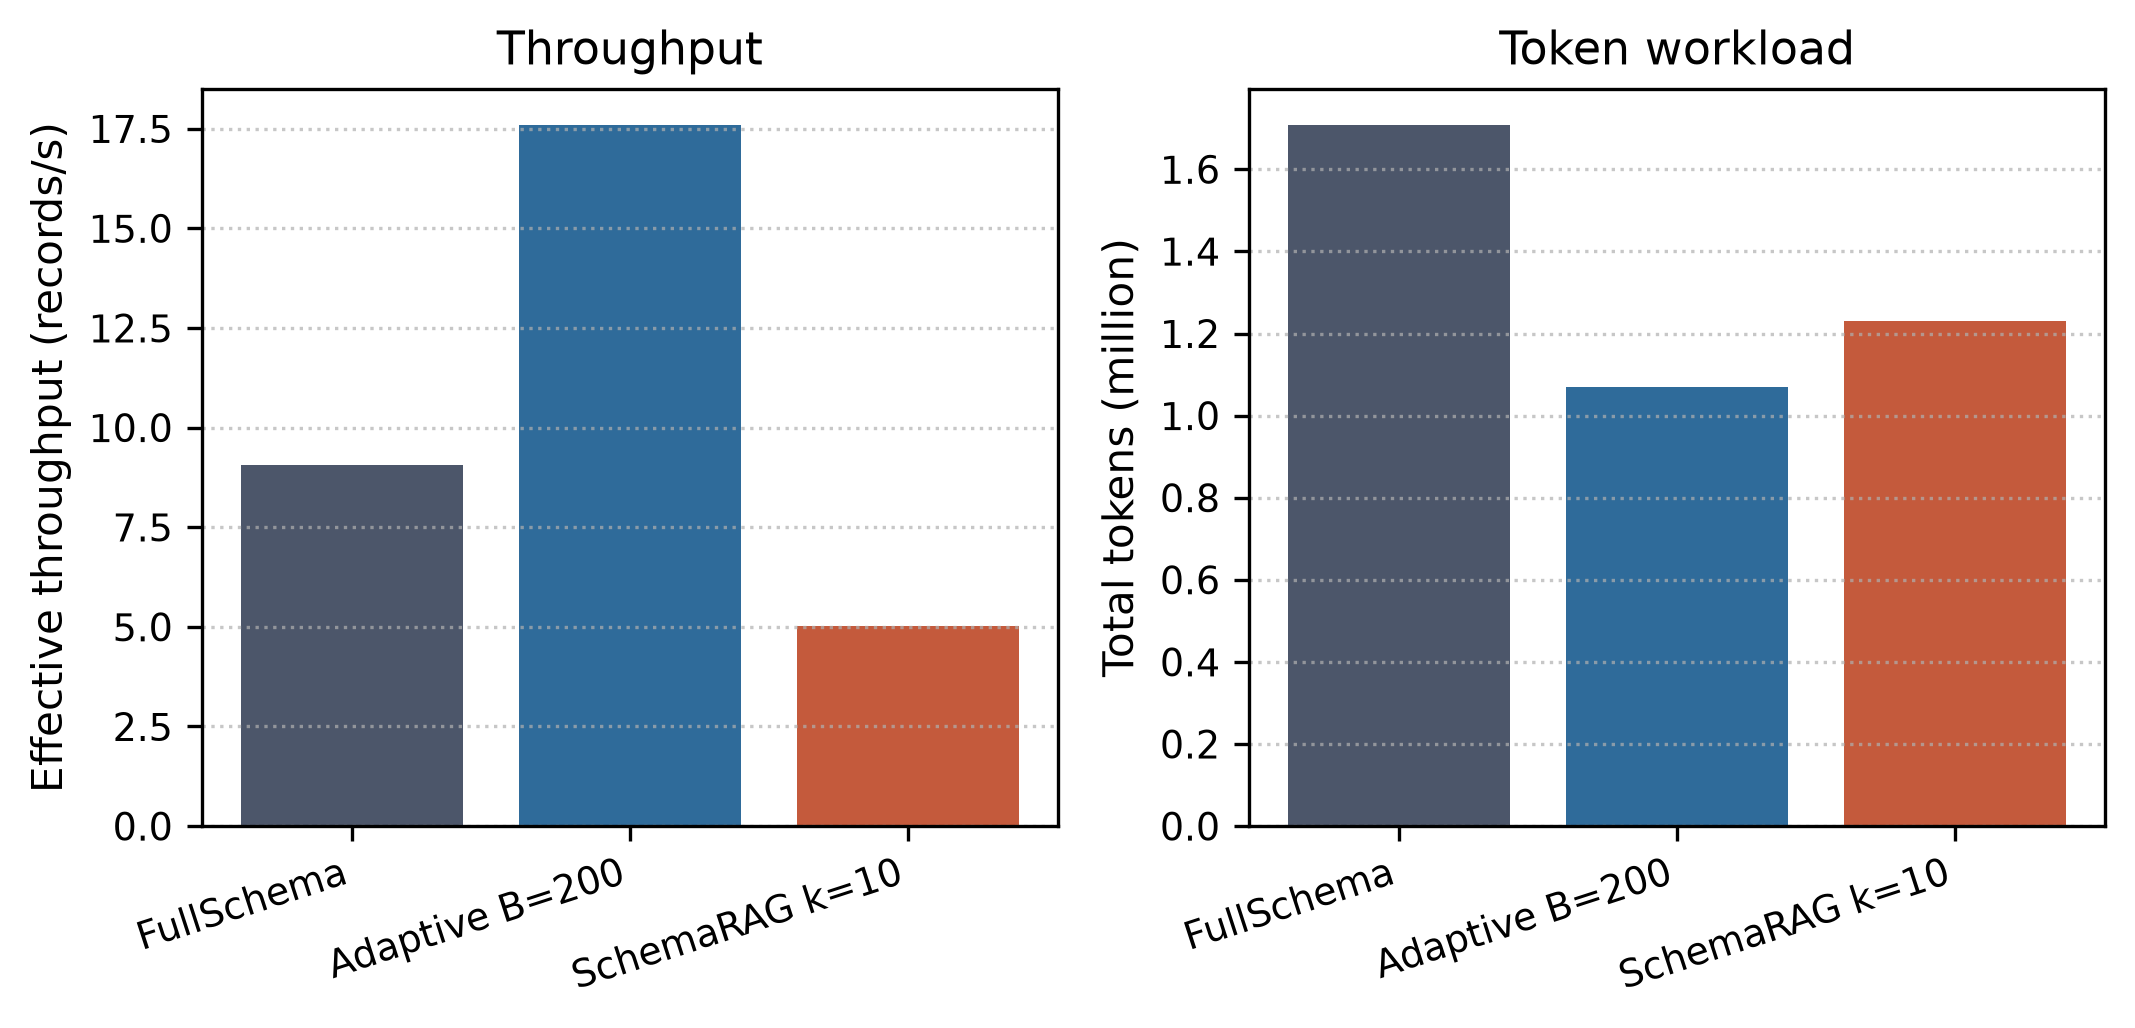
\includegraphics[width=.47\linewidth]{main_throughput_and_tokens.png}\hfill
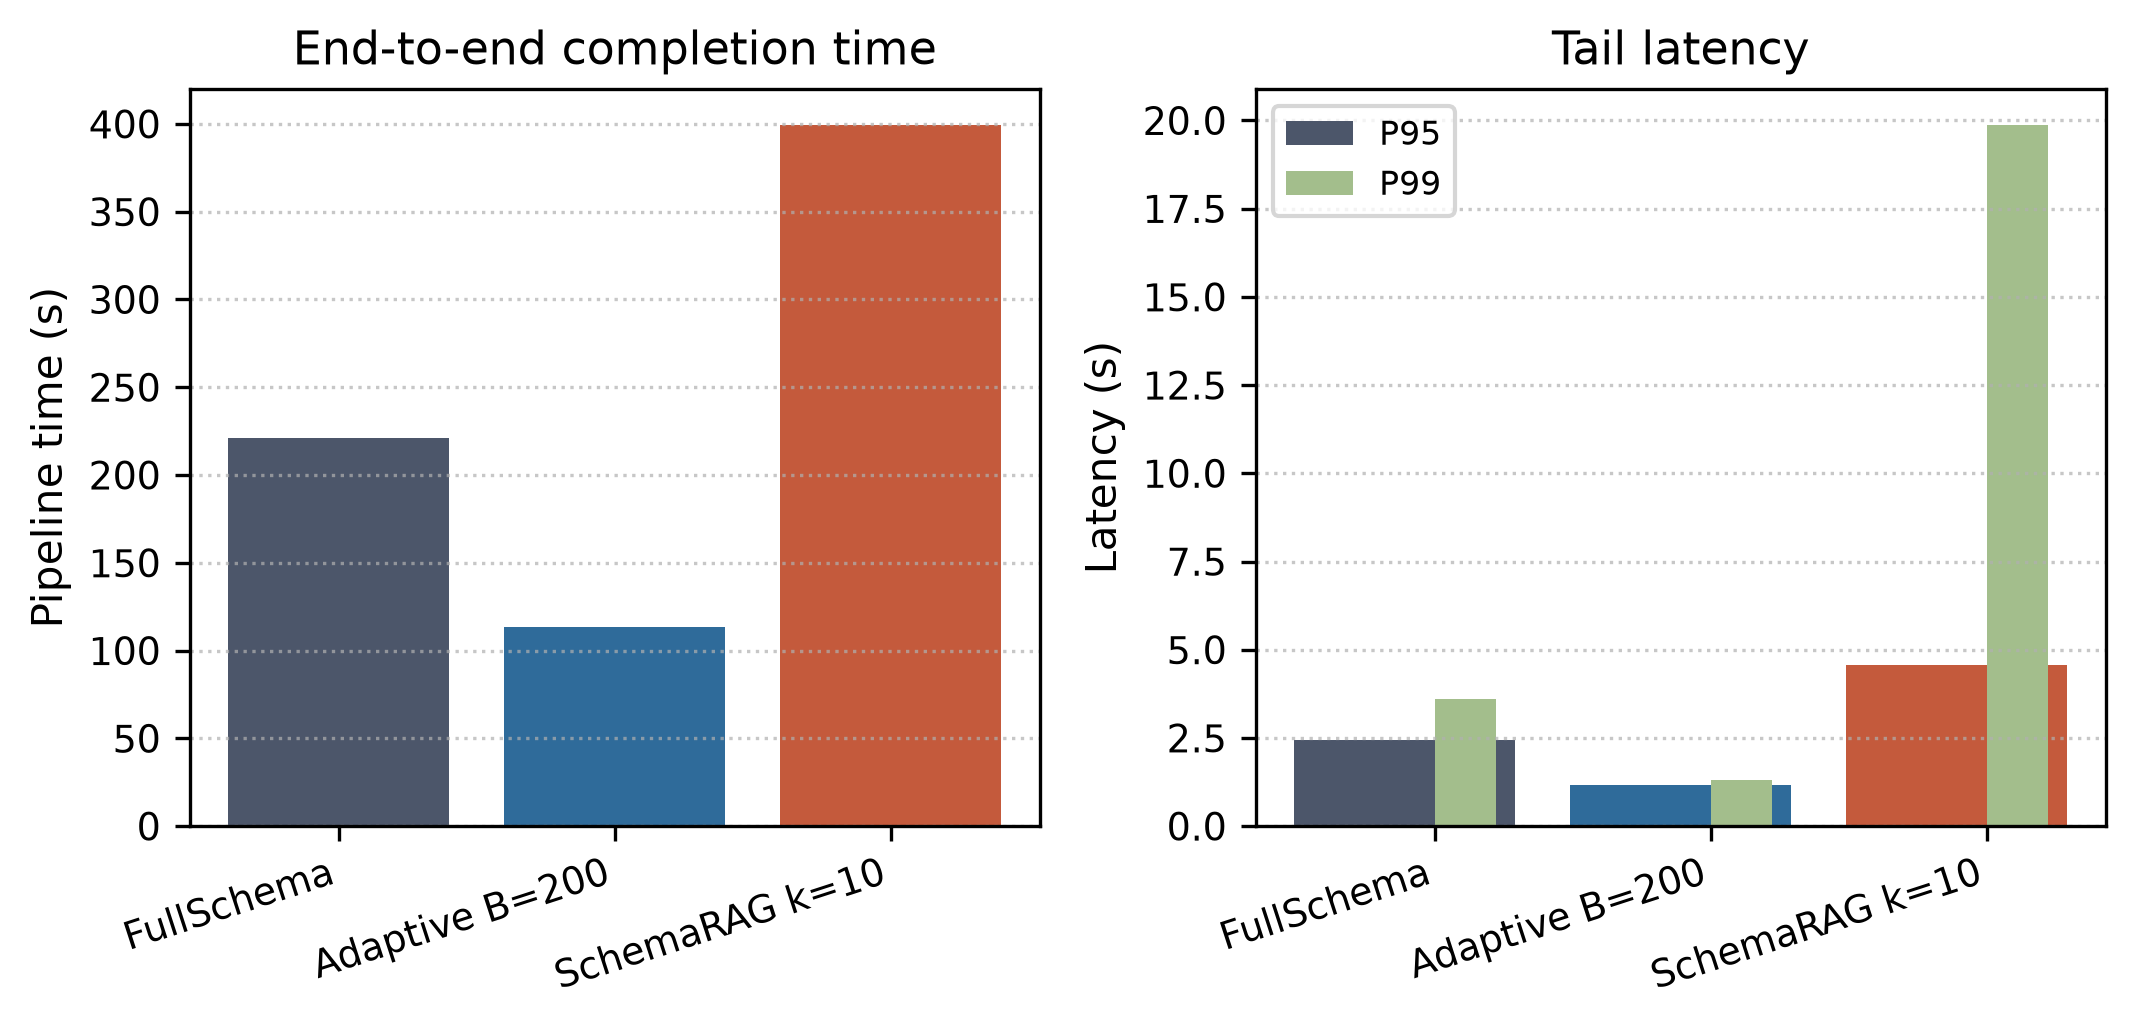
\includegraphics[width=.47\linewidth]{main_time_and_tail_latency.png}
\caption{Main online comparison on the 2,000-record development-distribution workload. The panels show
effective throughput, LLM token workload, makespan, and P99 latency for the three-run main experiment;
the comparison is limited to the stated model service and concurrency configuration.}
\label{fig:system-main}
\end{figure}

三次均值显示，`budget-200` 较 `full` 用时和 Token 更低、吞吐更高；两者时间的 95\% t 区间为
106.94--120.35 s 和 216.85--224.80 s。吞吐按每次运行计算后取均值，非表中均值相除；逐次值见
随稿材料。P99 含失败与重试并先逐次计算；三方法 P95/P99 均值分别为 2,438/3,601、
1,161/1,308 和 4,572/19,886 ms，显示外部适配尾延迟较高。三次合计每方法 6,000 个任务：
`full` 与 `budget-200` 无失败或重试；SchemaRAG 最终失败 6 条、重试 12 次，错误均为输出目标外键。
`Total tokens` 含 LLM 输入、输出和重试，不含 embedding；输入/输出均值分别为
1,399,176/309,926、939,791/129,463 和 1,019,842/210,569。

\subsection{预算响应与补充在线基线}

在相同 2,000 条冻结负载及 $c=16,q=16$ 下，进一步对九个预算点各作一次诊断性扫描。
表~\ref{tab:budget-response}中的字段比例是选中字段数占 18 个候选字段的比例，不是
表~\ref{tab:coverage}的参考字段覆盖率；Token 是实际 LLM 输入与输出之和，预算仍只是选择阶段容量。

\begin{table}[htbp]
\centering
\scriptsize
\setlength{\tabcolsep}{3pt}
\caption{Single-run online budget response on the 2,000-record frozen workload.}
\label{tab:budget-response}
\begin{tabular}{@{}rrrrrr@{}}
\toprule
Budget & LLM Token/record & Fields/record & Fields/18 (\%) & P99 (ms) & Success (\%)\\
\midrule
60   & 326.7 & 2.80 & 15.5 & 1240 & 100.00\\
100  & 404.0 & 4.15 & 23.1 &  993 & 100.00\\
150  & 482.4 & 5.90 & 32.8 & 1186 &  99.95\\
200  & 534.6 & 7.52 & 41.8 & 1445 & 100.00\\
300  & 627.4 & 10.13 & 56.3 & 1706 & 100.00\\
400  & 730.7 & 13.73 & 76.3 & 2818 & 100.00\\
600  & 856.1 & 18.00 & 100.0 & 3883 & 100.00\\
800  & 857.6 & 18.00 & 100.0 & 3870 & 100.00\\
1200 & 858.0 & 18.00 & 100.0 & 3915 & 100.00\\
\bottomrule
\end{tabular}
\end{table}

实际 Token 和字段数随预算总体增加，并在预算约 600、全部 18 个字段均被选中后饱和；P99
总体上升但并非逐点单调。`budget-200` 因而只是预设的中低容量 operating point，不是从曲线中
选出的全局最优点，也不能由 41.8\% 的字段比例推断参考字段完整性。

从 60 到 400 的区间，字段负载和实际 Token 持续增加，而 600 之后继续放宽容量已不再减少 Schema；
这为按可接受负载选择运行点提供了经验范围，而非给出唯一预算。结合表~\ref{tab:coverage}的遗漏率，
部署时应先确定可接受的字段选择缺失，再在对应预算区间内权衡 Token、尾延迟和成功率。

单次补充基线中，$\lambda=0.003$ 与 `prompt-omit/null` 的 LLM Token/record 为
625.5/823.2/892.6，P99 为 3575/2542/3903 ms。Prompt-only 对照仍使用全部字段，说明 Token
下降主要来自字段数缩减，尚未证明 M1 排序优势。以上均为单次结果；随机/频率 Top-$k$ 在线结果
仍缺失。

\subsection{端点方向性验证}

为拆分并发度和队列容量的方向性影响，另在 500 条记录上进行两组扫描：固定 $c=16$ 时取
$q\in\{4,8,16,32,64\}$，固定 $q=16$ 时取
$c\in\{1,2,4,8,16,32\}$。各点均为 `budget-200`，成功数为 500/500。
固定 $c=16$ 时吞吐依次为 21.04、21.31、21.54、20.20、21.01 条/s，队列等待 P99
依次为 578、758、997、1,908、3,265 ms；固定 $q=16$ 时吞吐依次为 1.67、3.34、
6.52、11.80、21.54、30.19 条/s。$q=64$ 的首次运行因 shell 超时仅提交 182 条，已用
干净重跑提交 500 条的结果替代，不将首次中断计入扫描结论。

固定 $c$ 时增大 $q$ 主要抬高队列等待尾部而无稳定吞吐增益；固定 $q$ 时增大 $c$ 可提高吞吐，
但高并发会抬高尾延迟。完整端点结果见随稿材料。该扫描仍限于单进程，不能推出生产规模扩展性，
也说明系统优化不能只最小化 Token，还需同时观察时间、成功率和尾延迟。

\subsection{初始化成本边界}

100 条 M1 隔离训练耗时 737.13$\pm$43.69 ms，模型 3.36 MB，冷加载
178.26$\pm$14.43 ms。100 条本地规划批次耗时 366.63 ms；独立阶段测量为
3.09$\pm$0.16 ms/条，完整 planning 加 prediction 与 Prompt 构造约 6.2 ms/条，二者口径不同。
按已测一次性启动 915.39 ms 和在线差异，budget--full 时间 break-even 约 17 条，Token 维度为
0；SchemaRAG 在当前范围内未获得时间收益。该估算不含启动样本生成、环境启动和冷缓存等，
不是货币成本或完整生命周期审计。

\section{讨论}

本文的在线实验表明，在当前单进程流水线和服务配置下，`budget-200` 与较低 Token、较短
makespan 和较高有效吞吐相关；SchemaRAG 的结果也表明，检索开销可能抵消字段负载减少带来的
收益。因此负载整形应以字段选择完整性、端到端时间、吞吐、成功率和尾延迟共同观察。

就工程含义而言，本文验证的是将 Schema 负载显式限制在可审计预算内，并测量这一限制对在线流水线
的影响；它并未证明被保留字段具有最优排序，也未证明遗漏字段在具体业务中不重要。这样的边界使预算
能够作为部署约束参数，而不是被表述为替代事实质量评估或通用字段重要性判断的代理量。
476 条共享成功子集上的选择缺失率揭示了 `budget-200` 的完整性代价，但本文没有验证字段值
的事实正确性，因而不据此声称端到端事实质量等价或优于 `full`。预算扫描确认字段数和实际 LLM
Token 可由容量调节并最终饱和，但近似字段数基线与离线消融均未显示当前 M1 加权背包具有稳定
优势。因此，本文可归因的主要机制是预算约束下的字段负载控制，而非现有排序或手工权重的最优性。

当前参考并非人工事实 Gold；性能负载来自开发分布；SchemaRAG 为外部重实现；系统和并发扫描均为
单进程；在线统计不含启动样本生成等生命周期成本；新增预算与基线点仅运行一次，且缺少随机/频率
Top-$k$ 的在线比较。后续需在人工验证参考、未见负载、按近重复簇隔离、跨模型数据及多进程环境中
重评估。

\section{结论}

本文提出并评估了由 FullSchema 模型辅助银标训练的预算感知动态 Schema 选择流程。在当前
模型、单进程 Runner、$c=16,q=16$ 和 2,000 条开发分布性能负载条件下，M1 `budget-200`
与较低 Token、较短流水线时间和较高有效吞吐同时出现；在 500 条模型辅助评价参考记录的 476 条共享成功子集上，它的
参考字段覆盖率为 83.03\%，选择缺失率为 16.97\%。因此结果表明的是效率与字段选择完整性之间
的显式工程权衡，而不是无损裁剪。预算曲线支持以容量控制字段负载，但在线近似字段数基线和离线
消融表明，Token 收益主要来自字段数缩减，当前 M1 排序和手工权重未表现出稳定最优性。该参考不验证
字段值事实质量，结果也不支持通用最优性、独立泛化或生产级扩展性结论。

\section*{数据、代码与结果来源}

原始记录受授权、版权和隐私约束，受限数据可合理申请。实验所用 LLM 和 embedding 服务均部署于机构内网，
原始记录未发送至外部云服务。可发布的派生数据、实验配置、分析脚本和
结果归档将在论文发表时通过代码仓库提供。归档材料包含主实验与离线诊断的结果、配置哈希和复现实验
命令；外部服务端版本无法由本地归档冻结。

\bibliographystyle{splncs04}
\bibliography{references}

\end{document}
